\section{Mass transfer via RLOF by the outer star}\label{sec:mass_transfer_RLOF}

In this section, I describe how mass transfer by the outer star towards the inner binary affects the evolution of the system. Despite the fact that I discuss the first model listed in \cref{tab:simulations_settings}, the general picture is similar for all models. In the next sections, I explicitly compare and analyse the differences between the models listed in \cref{tab:simulations_settings}.

On one hand, no remarkable mass transfer takes places during the first four years of the simulation. On the other hand, the tertiary's envelope experience a series of significant deformations during that same period due to the combined effect of two factors. First, the outer orbit is eccentric, see \cref{tab:system_orbit_param}, and second, I use a collection of particles to represent the outer star. The latter means that the giant's spherical symmetry is disturbed close to the pericenter and it is restored close to the apocenter. This is effectively the result of tidal interactions between the two orbits, which is a dissipative process and shrinks the outer orbit. In \cref{fig:simualtion_snapshots}, I present four snapshots of the system's evolution at $t = 3.75, \; 5, \; 6.25$ and $7.5$ yr. The envelope's deformation is evident by comparing the system at $t = 3.75$ yr, when the tertiary approaches the orbit's apoecenter, to $t = 6.25$ yr, when it approaches the orbit's pericenter.
\begin{figure}[H]
    \centering
    \begin{subfigure}[b]{0.49\textwidth}
        \centering
        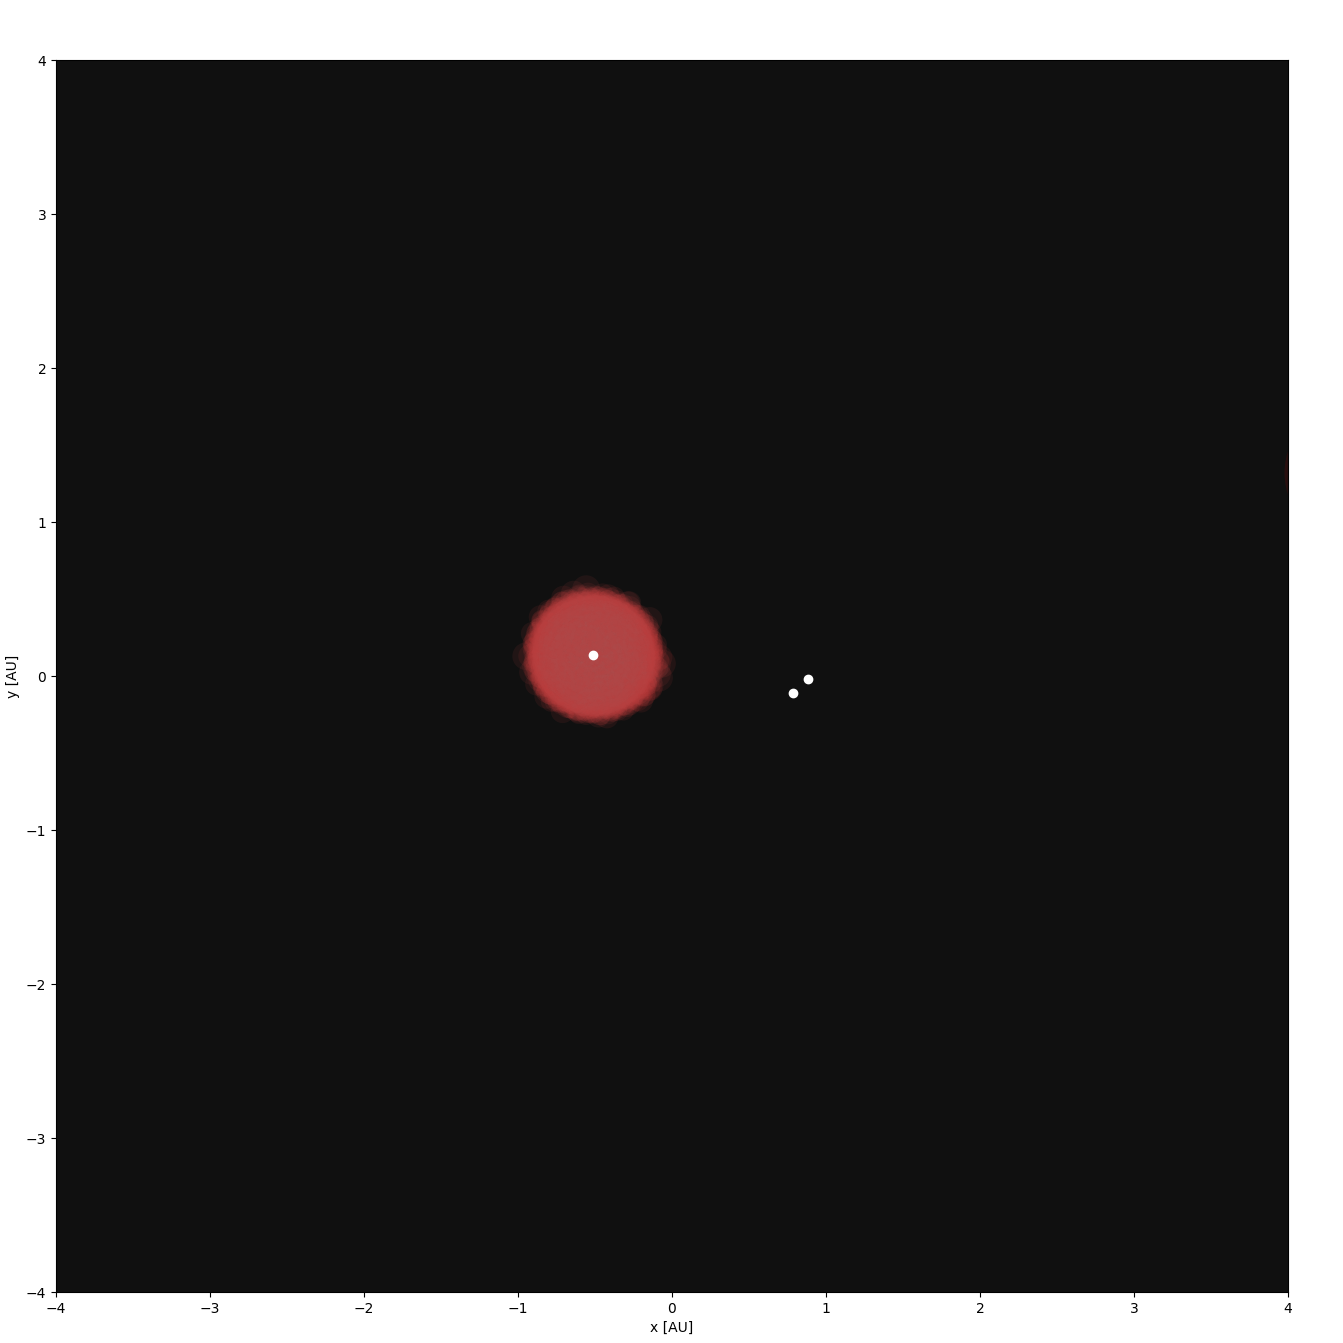
\includegraphics[width=\textwidth]{Thesis/graphs/hydro_triple_small0013687.png}   
    \end{subfigure}
    \hfill
    \begin{subfigure}[b]{0.49\textwidth}  
        \centering 
        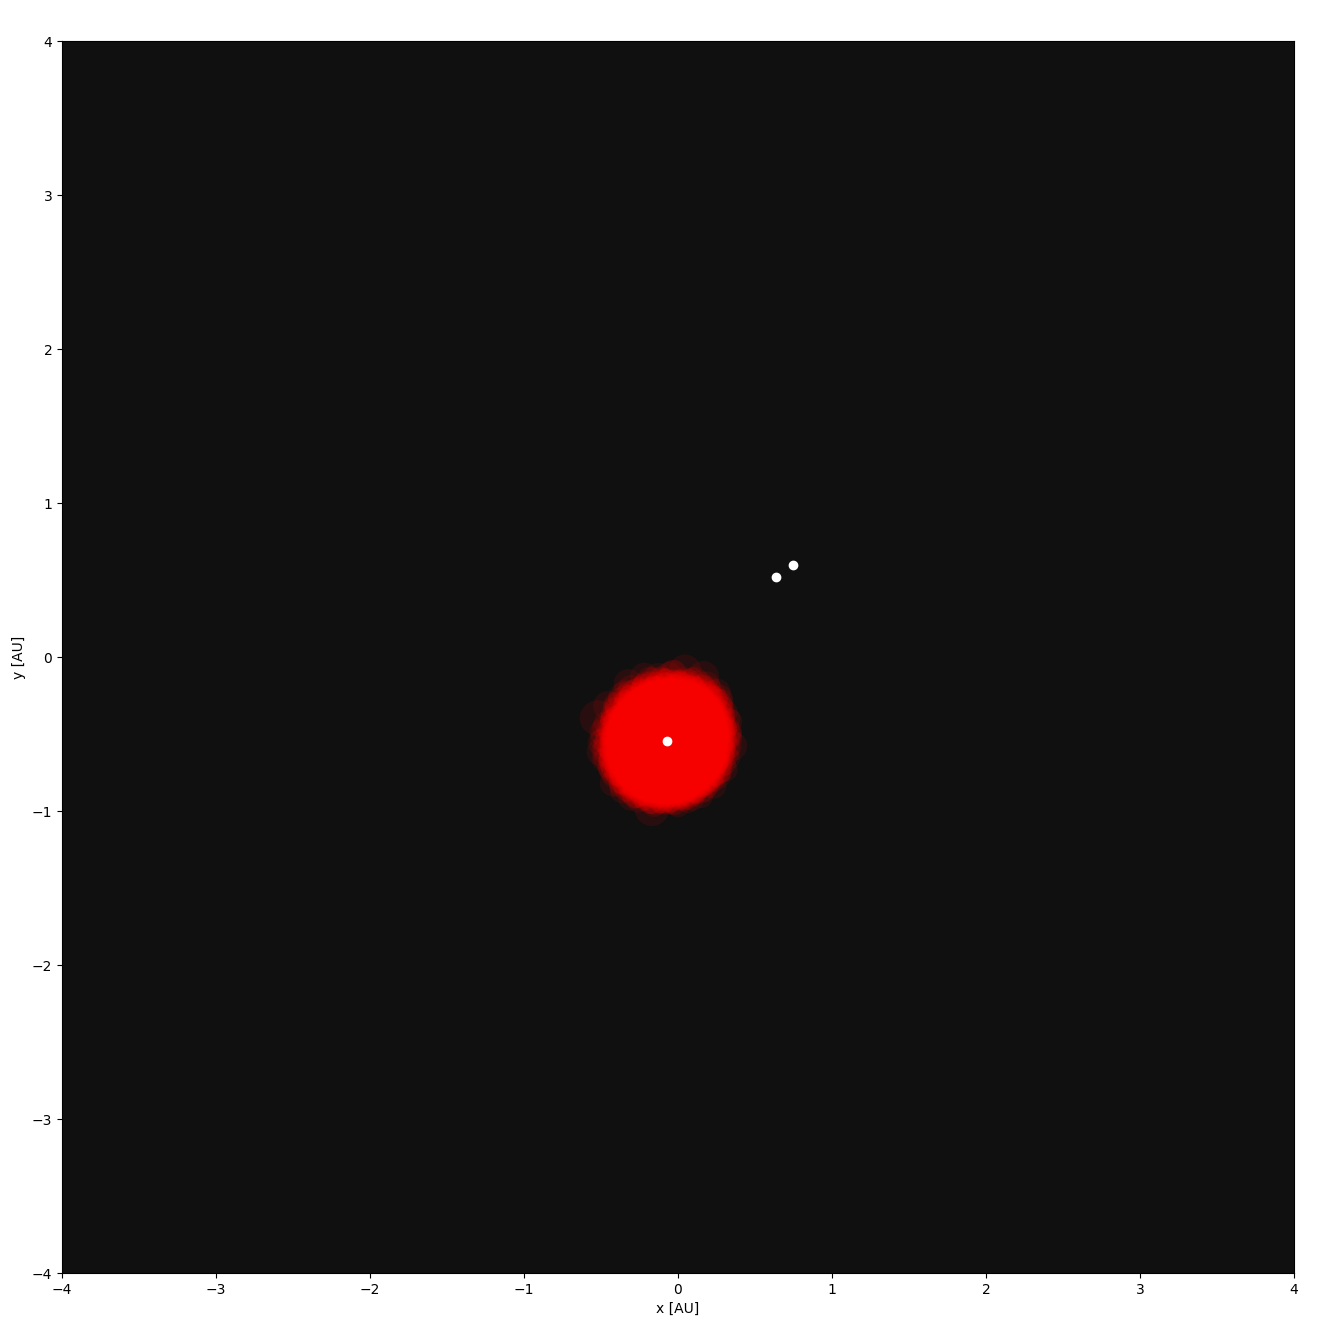
\includegraphics[width=\textwidth]{Thesis/graphs/hydro_triple_small0018250.png}
    \end{subfigure}
    \vskip\baselineskip
    \begin{subfigure}[b]{0.49\textwidth}  
        \centering 
        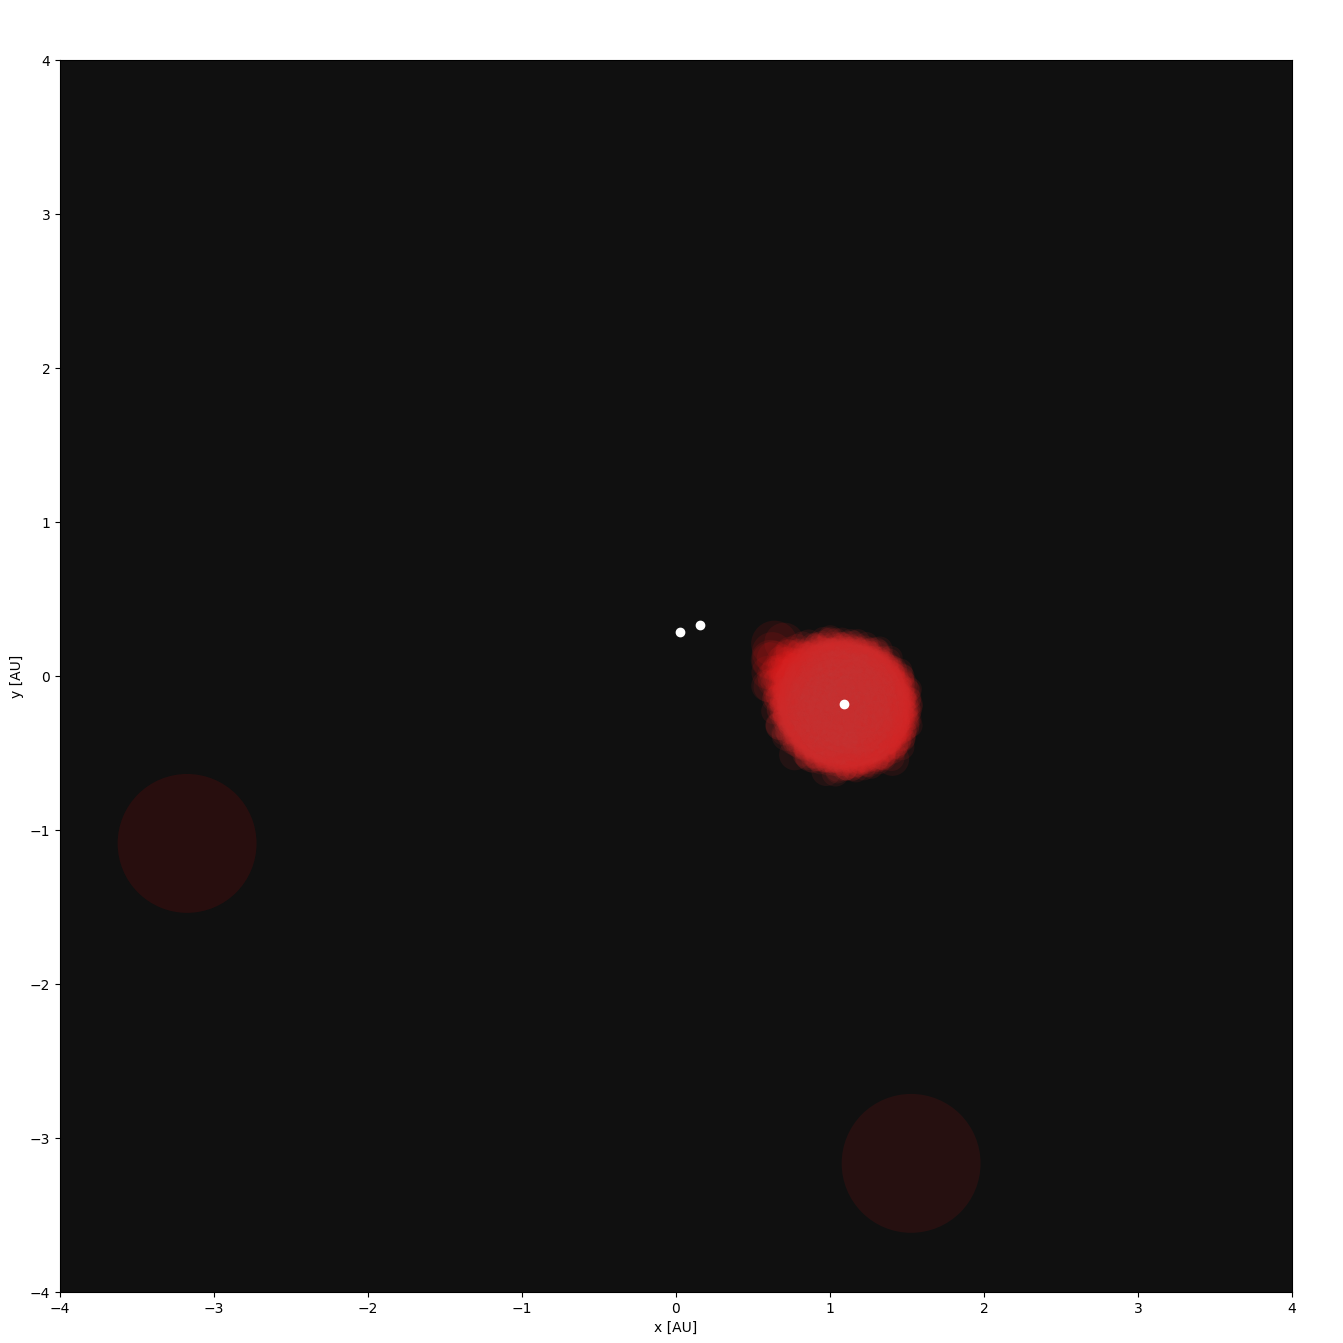
\includegraphics[width=\textwidth]{Thesis/graphs/hydro_triple_small0022812.png}
    \end{subfigure}
    \hfill
    \begin{subfigure}[b]{0.49\textwidth}  
        \centering 
        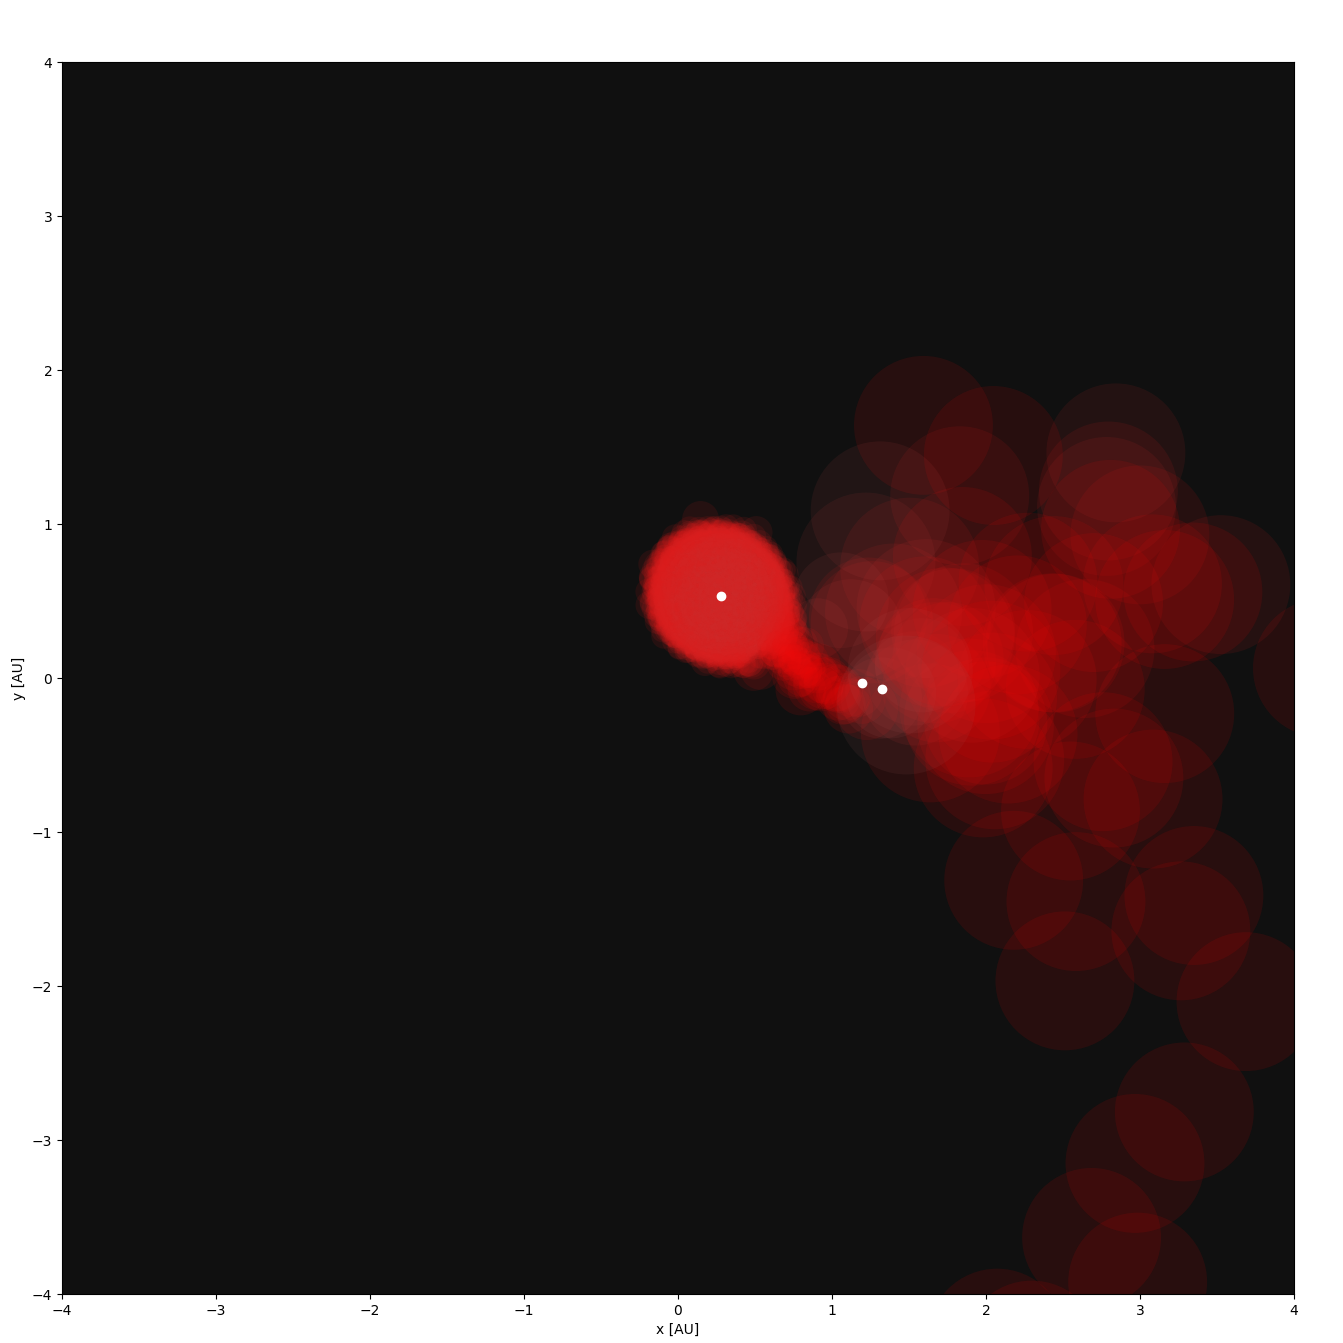
\includegraphics[width=\textwidth]{Thesis/graphs/hydro_triple_small0027375.png}
    \end{subfigure}
    \caption{System snapshots, from top to bottom and left to right, at 3.75, 5, 6.25 and 7.5 yr}
    \label{fig:simualtion_snapshots}
\end{figure}
Significant mass transfer from the tertiary towards the inner binary begins at $t \approx 4$ yr, so the time period of interest for my work begins at that point. The mass loss from the outer giant is periodic, modified by the outer orbit's periodicity, see \cref{fig:accretion_inc_00_mass_loss}. This is due to the slightly eccentric outer orbit, which causes the giant to overfill its Roche lobe at pericentre, but after semilatus rectum, the star detaches from its Roche lobe, to re-establish RLOF when it reaches pericentre again. As a result, the aforementioned periodicity is intrinsically carried through the evolution of the tertiary's mass too, see \cref{fig:accretion_inc_00_mass_loss}. Additionally, there is a significant delay between the moments of pericentre crossing and the maxima in mass transfer, see \cref{fig:simualtion_snapshots}, which is consistent with a study of RLOF in eccentric binaries \citep{lajoie2010mass}.
\begin{figure}[!htb]
    \centering
    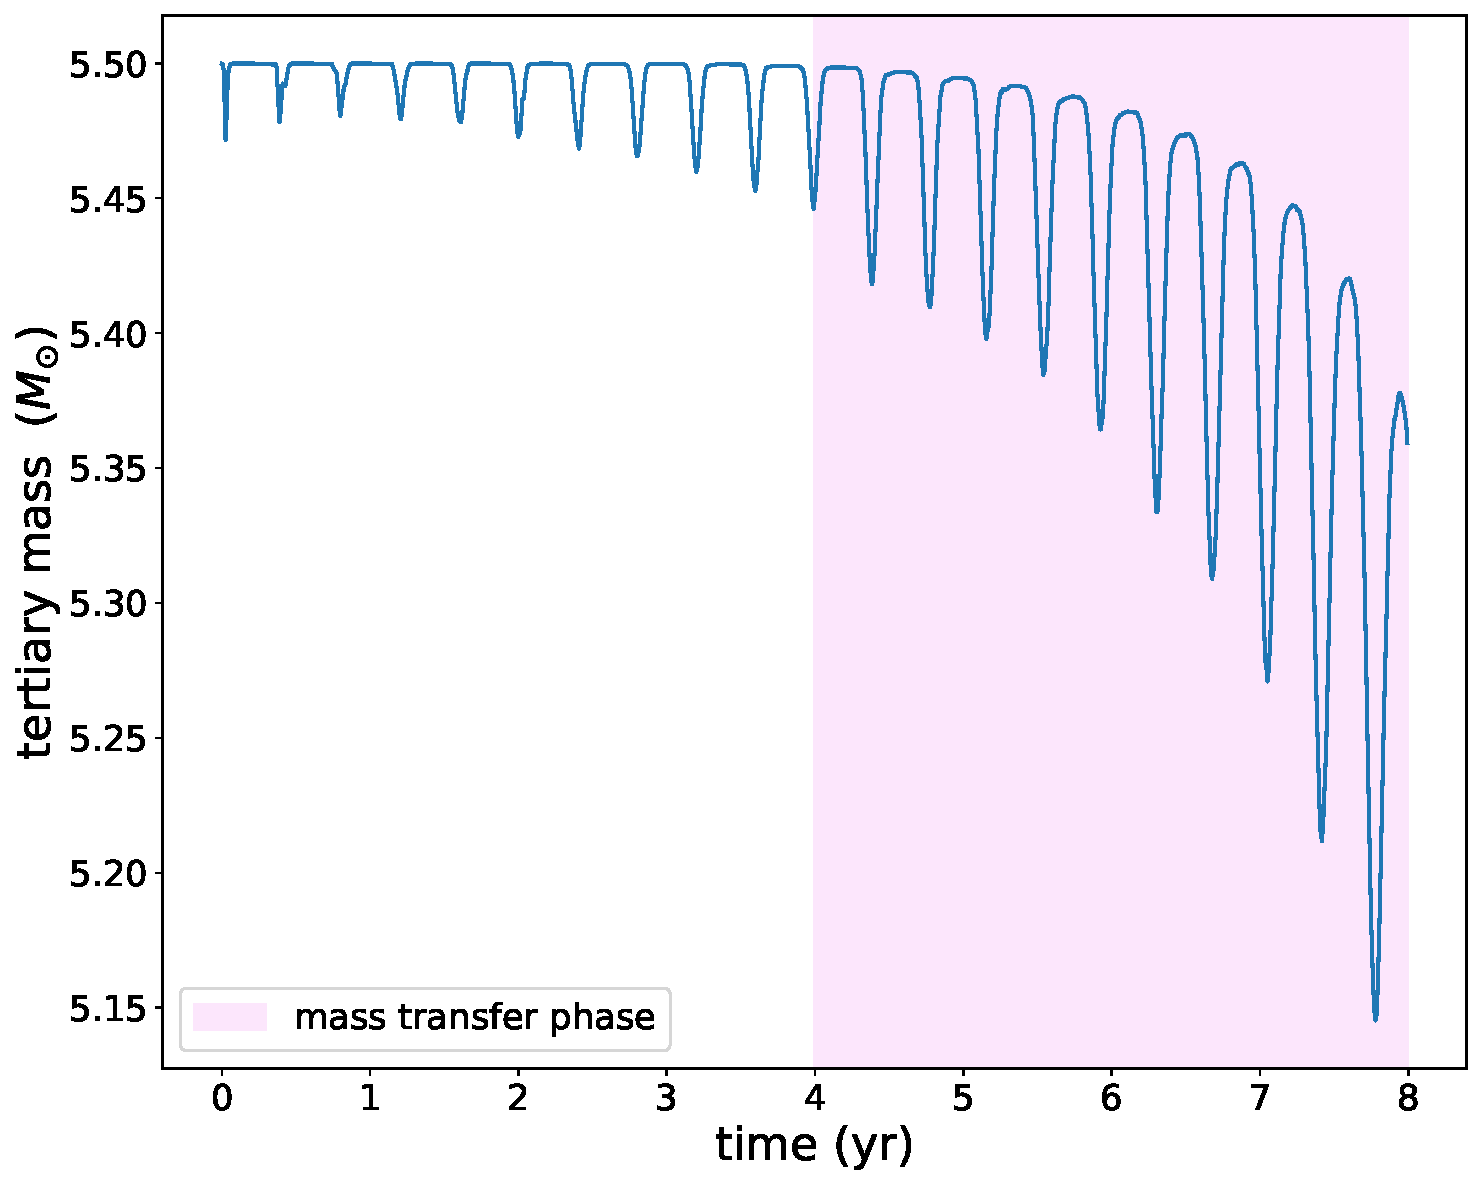
\includegraphics[width=0.85\textwidth]{Thesis/graphs/inc_00/accretion_inc_00_mass_loss.pdf}
    \caption{The evolution of the tertiary's mass.}
    \label{fig:accretion_inc_00_mass_loss}
\end{figure}
The mass transfer becomes progressively unstable, as expected for a donor with a convective envelope. Furthermore, the mass flowing from the first Lagrangian point of the outer orbit to the inner binary system interacts with the paths of the binary components. As a result, instead of a circumbinary disk, a gaseous cloud, similar to a common envelope (CE) \citep{ivanova2013common}, develops around the binary, see \cref{fig:simualtion_snapshots}. Part of the mass is accreted by the inner binary and the rest escapes the system through the third Lagrangian point of the outer orbit, see \cref{fig:simualtion_snapshots}.

After eight years, which corresponds to $\approx 20$ orbits of the tertiary, the system enters the unstable regime, see \cref{eq:stability_regime}, and thus I terminate the simulations. Every $\delta t_{bridge}=0.1$ day, see \cref{tab:codes_settings}, I extract the mass, position and velocity of each particle in the computational domain. These properties are used to calculate the orbital parameters of the inner and the outer orbits. More specifically, the semi-major axis and eccentricity of the inner orbit are calculated using the relative position and velocity of the inner binary components. Furthermore, the relative position and velocity of the inner binary center of mass and the tertiary are used to determine the semi-major axis and eccentricity of the outer orbit. The calculations are based on \cref{eq:semi-major_axis} and \cref{eq:eccentricity}, where $M = M_1 + M_2$ and $M = M_1 + M_2 + M_3$ for orbital parameters of the inner and outer orbit, respectively. Finally, I calculate the outer orbit's relative inclination with respect to the inner orbit, i.e. mutual inclination, as the angle between their respective orbital angular momentum the vectors.

Despite being out of the scope of this work, it is worth noticing, that shortly after $t=8$ yr, the mass transfer becomes extremely unstable and a triple common envelope is encountered in all cases except for model number 3 listed in \cref{tab:simulations_settings}. For the rest models, the remainder of the tertiary's envelope engulfs the inner binary and the tertiary's core. In the case of $i_{mut} = 20^{\circ}$, the core of the tertiary is ejected from the system leaving behind a high eccentric binary. Finally, in both cases where the two orbits are initially coplanar, a direct collision completely disrupts the system.

\subsection{Outer orbit}

Tidal effects between the two orbits dominate the rates of change of orbital parameters up to $t \approx 4$ yr. The effect of mass transfer becomes visible after $t \approx 4$ years. A portion of the transferred mass is accreted by the binary components, while the remainder is expelled from the system.  The ejected mass carries away orbital angular momentum, hence the outer orbit shrinks, see \cref{fig:accretion_inc_00_outer_semimajor_axis}. As a result,  the outer Roche lobe shrinks as well, see \cref{eq:roche_lobe}, and an increasing amount of mass can overflow towards the inner binary, see \cref{fig:accretion_inc_00_mass_loss}. 
\begin{figure}[H]
    \centering
    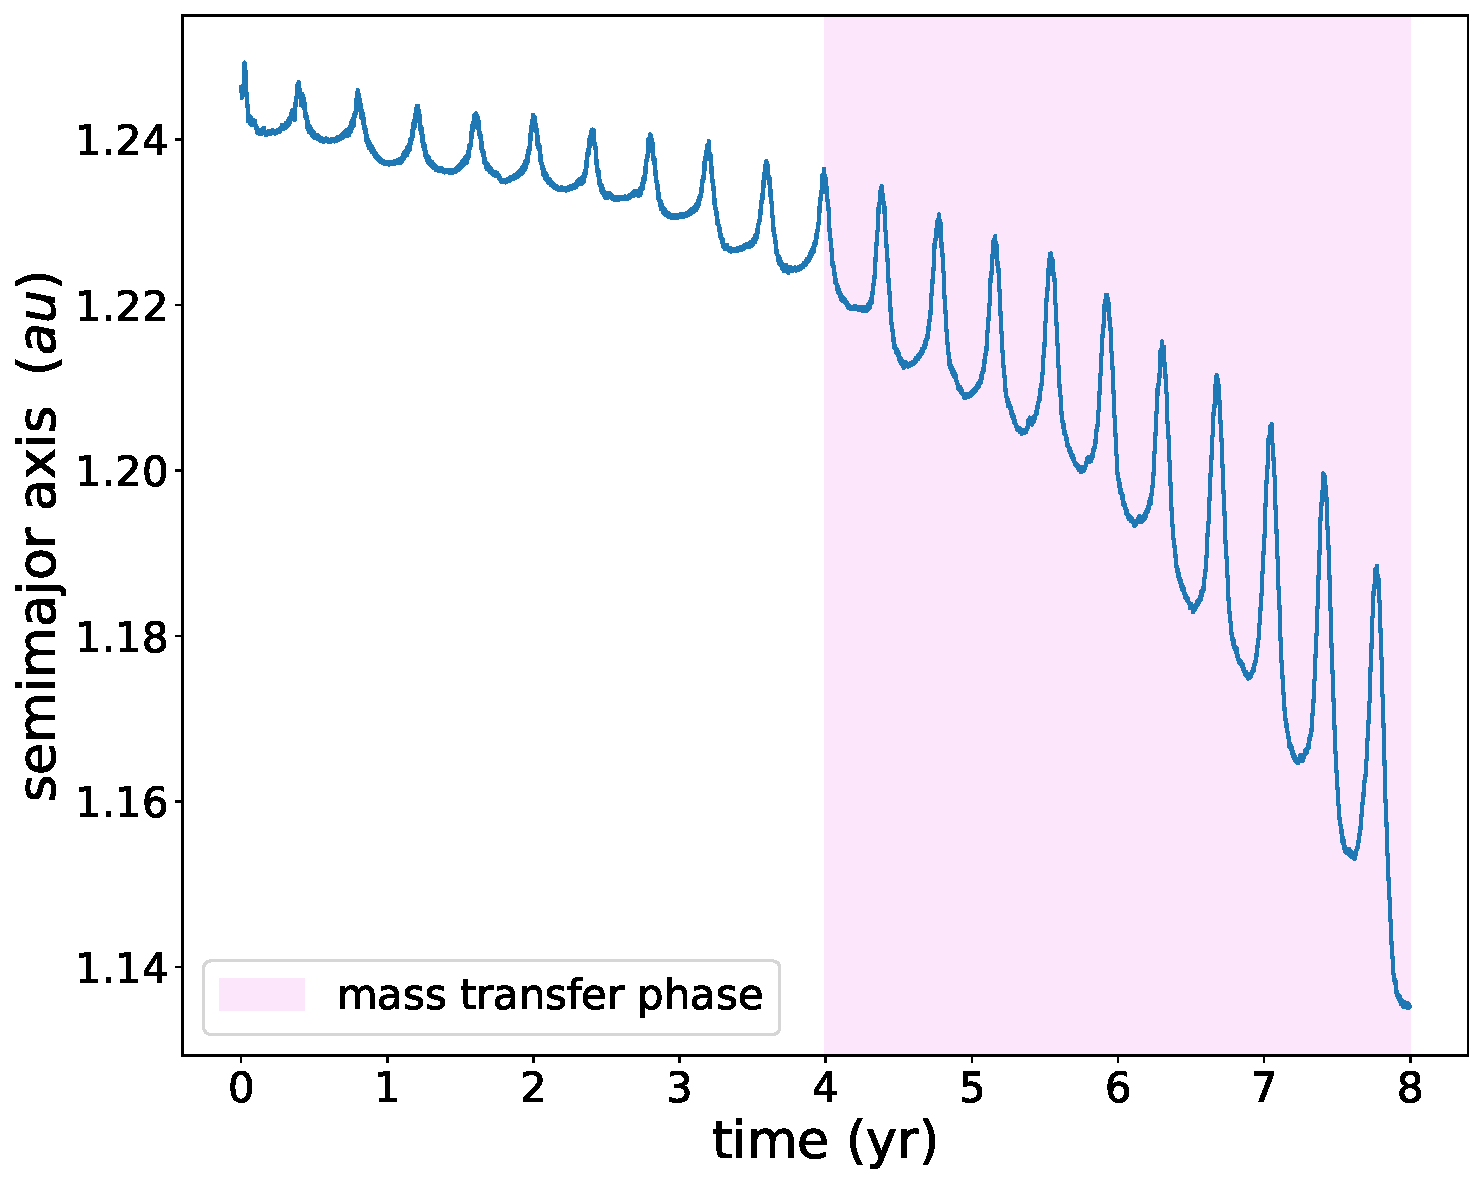
\includegraphics[width=0.85\textwidth]{Thesis/graphs/inc_00/accretion_outer_inc_00_semimajor_axis.pdf}
    \caption{Evolution of the semi-major axis of the outer orbit.}
    \label{fig:accretion_inc_00_outer_semimajor_axis}
\end{figure}
\begin{figure}[H]
    \centering
    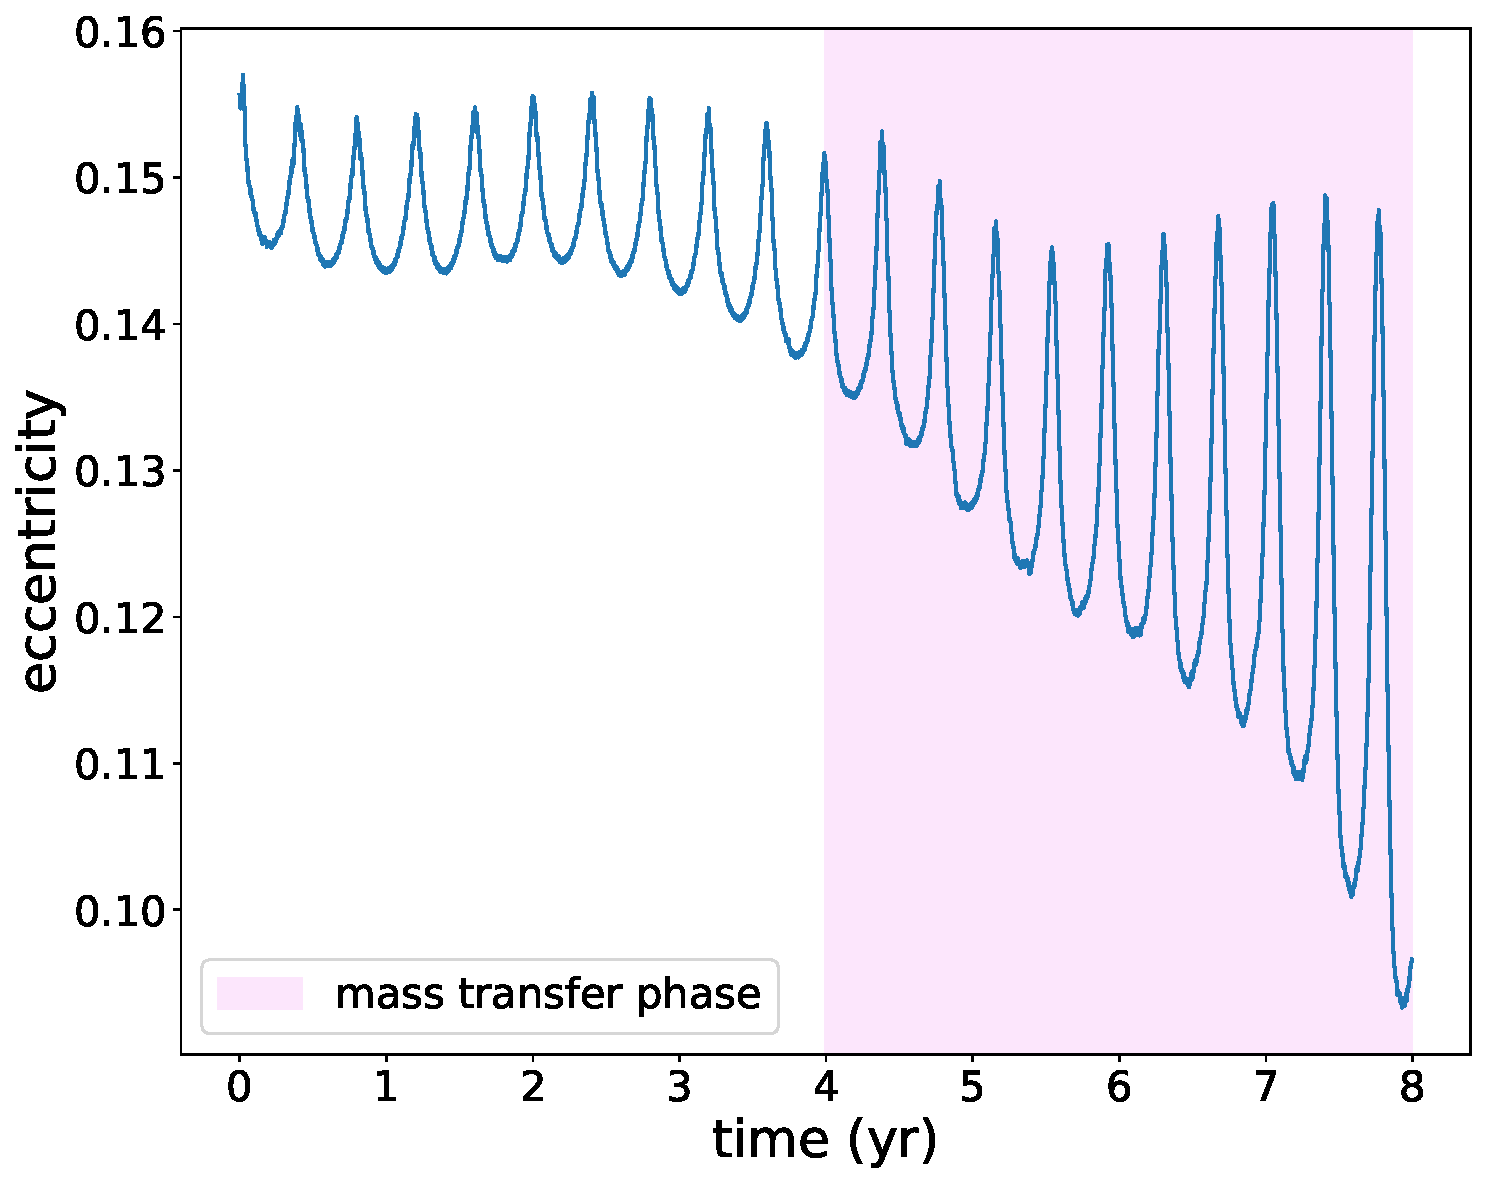
\includegraphics[width=0.8\textwidth]{Thesis/graphs/inc_00/accretion_inc_00_outer_ecc.pdf}
    \caption{Evolution of the eccentricity of the outer orbit.}
    \label{fig:accretion_inc_00_outer_ecc}
\end{figure}
\begin{figure}[H]
    \centering
    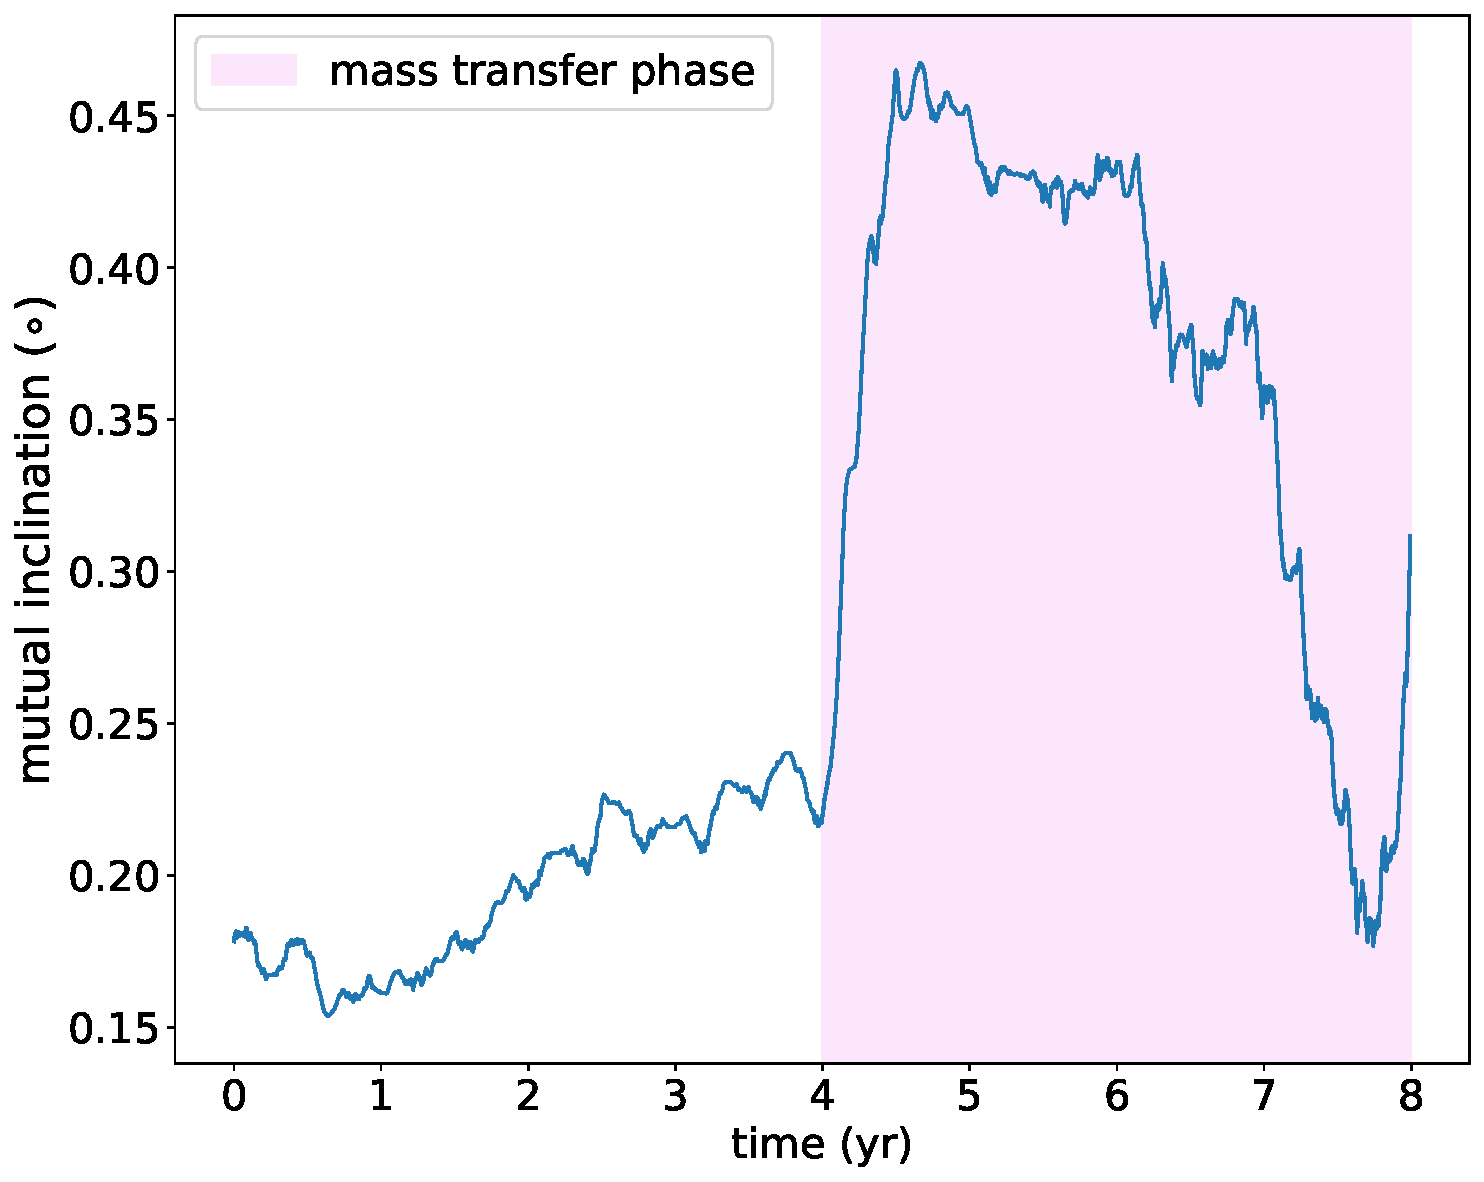
\includegraphics[width=0.8\textwidth]{Thesis/graphs/inc_00/accretion_inc_00_inc.pdf}
    \caption{Evolution of the inclination of the outer orbit relative to the inner orbit.}
    \label{fig:accretion_inc_00_inc}
\end{figure}
Furthermore, as the tertiary approaches the inner binary, tidal effects between the two orbits become stronger. Tides tend to circularize and flatten the outer orbit. \cref{fig:accretion_inc_00_outer_ecc} shows the former, while \cref{fig:accretion_inc_00_inc} shows the latter, where the outer orbit, which is already coplanar with the inner orbit, remains close to coplanarity.


\subsection{Inner orbit}

As the transferred mass intersects the inner orbit, the binary components interact with the gas. Some of the gas is accreted, while some is ejected from the binary's close vicinity. The inner binary is influenced by hydrodynamics, notably gas drag, which always tends to shrink the orbit, as well as the accretion process and the gravitational interaction of the inner orbit with the incoming material stream.  The effect of the later on the evolution of the orbit is complex and depends on the angle at which the mass stream crosses the inner obit. This is discussed in more detail in \cref{sec:inclination}. 

In \cref{fig:accretion_inc_00_inner_semimajor_axis} and \cref{fig:accretion_inc_00_inner_ecc}, I present the evolution of the semi-major axis and eccentricity of the inner orbit, 
respectively. Both graphs show the presence of the tertiary, which introduces the observed fluctuations with periods equal to the period of the outer orbit, $\Delta t \approx 145.5$ days.
\begin{figure}[H]
    \centering
    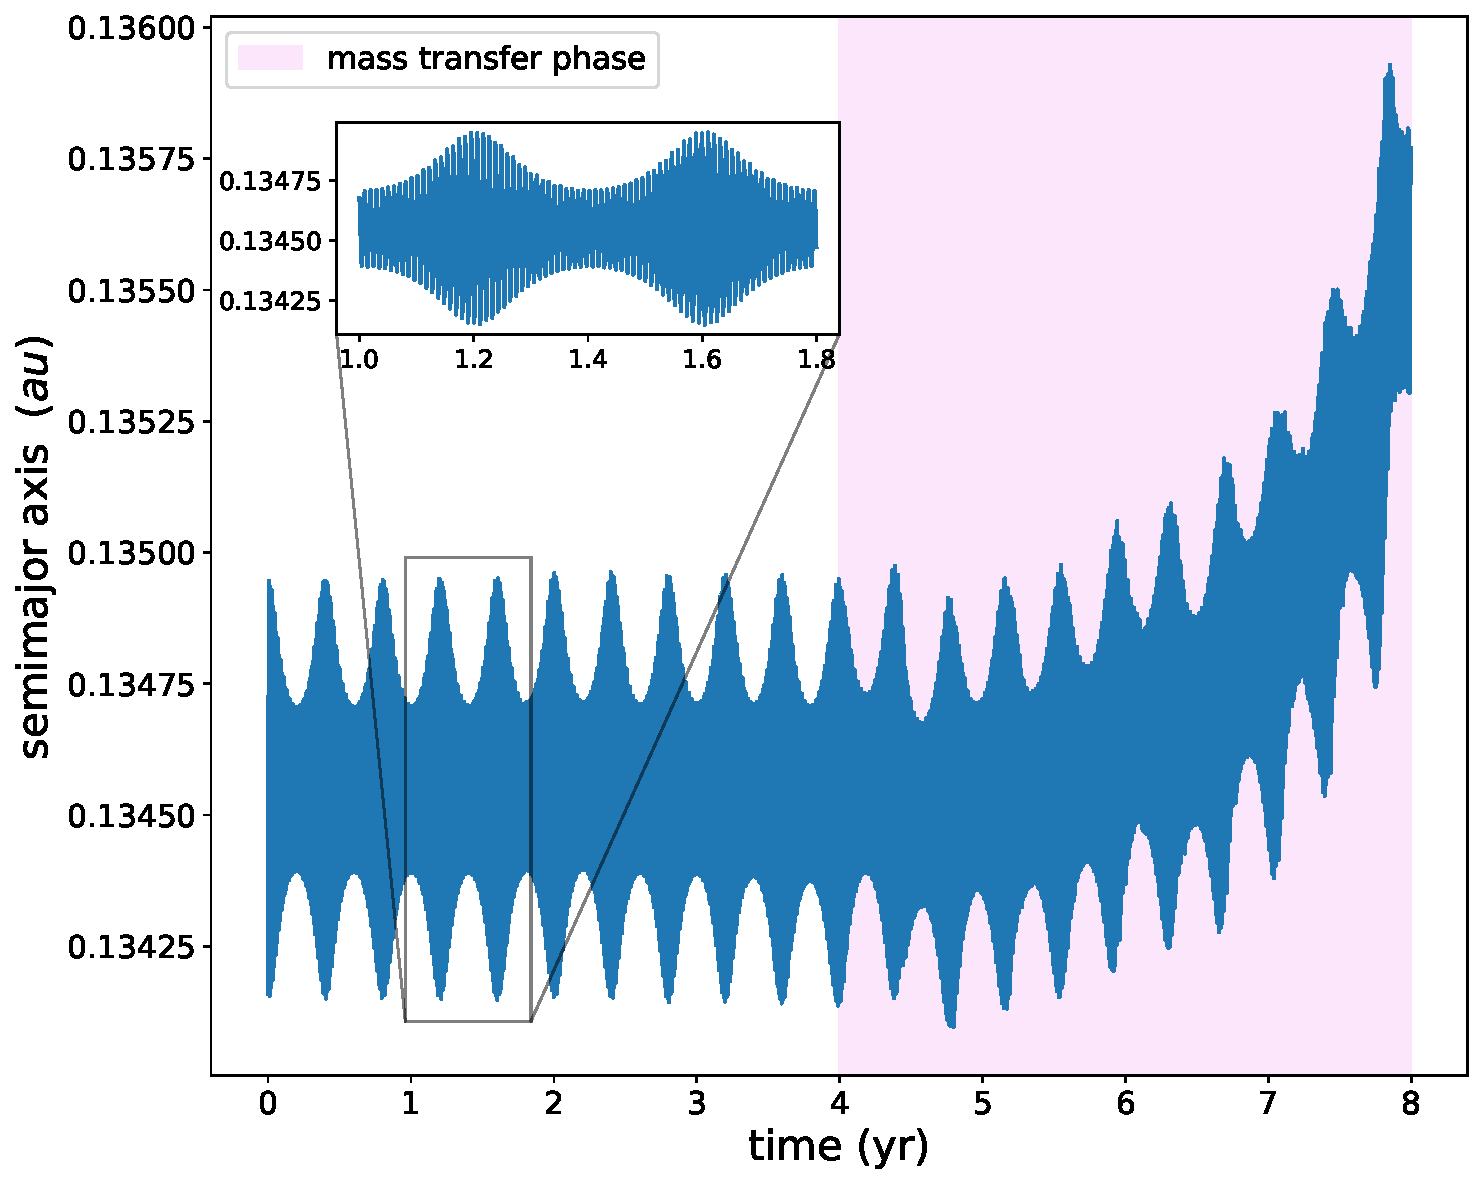
\includegraphics[width=0.9\textwidth]{Thesis/graphs/inc_00/accretion_inc_00_inner_semimajor_axis.pdf}
    \caption{Evolution of the semi-major axis of the inner orbit.}
    \label{fig:accretion_inc_00_inner_semimajor_axis}
\end{figure}
In the case where the inner and outer orbit are coplanar the former seems to widen, see \cref{fig:accretion_inc_00_inner_semimajor_axis}. This is an unexpected outcome since a common envelope-like structure around the binary is encountered. Friction between the rotating stars and the slow-rotating envelope is expected to shrink the orbit in the typical common envelope model, hence a detailed discussion regarding this this result is taking place in \cref{sec:resolution}. Finally, the effect of mass transfer on the eccentricity of the inner orbit is negligible and the orbit remains circular. 
\begin{figure}[!htb]
    \centering
    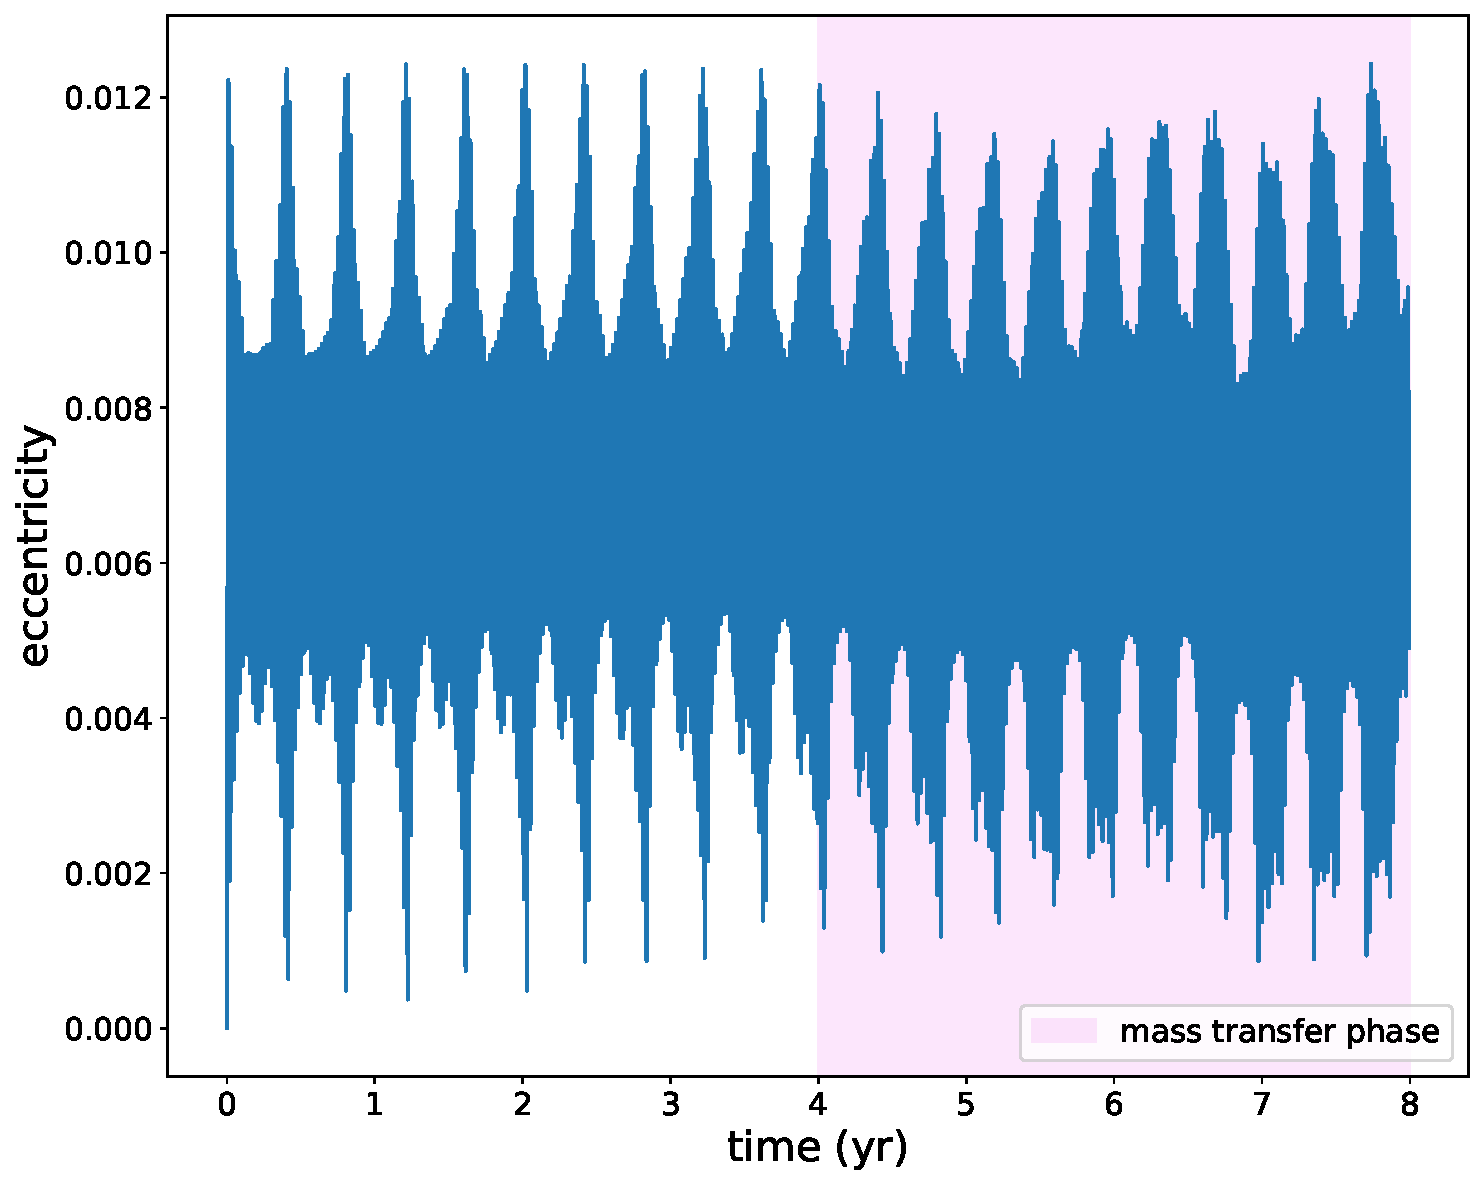
\includegraphics[width=0.9\textwidth]{Thesis/graphs/inc_00/accretion_inc_00_inner_ecc.pdf}
    \caption{Evolution of the eccentricity of the inner orbit.}
    \label{fig:accretion_inc_00_inner_ecc}
\end{figure}


